Multi-objective optimization is characterized by the presence of multiple, possibly conflicting, objectives. This means that the optimal solution for any single objective doesn't necessarily correspond to the optimal solution for the other objectives. What we get instead is a set of solutions that are optimal in the sense that no other solution is better in all objectives. This set of solutions is called the Pareto front.

The state of the art in multi-objective optimization is the NSGA-II algorithm, which is a genetic algorithm that uses a non-dominated sorting approach to create fronts of solutions that are not dominated by any other solution. The algorithm then selects the best solutions from the fronts, ensuring that the population is diverse and that the Pareto front is well represented (maximimization of the crowding distance).

\subsection{Kursawe Function}
The Kursawe function is a simple test function for multi-objective optimization. It is defined as follows:
\begin{equation}
    \begin{cases}
        f_1(x) = \sum_{i=1}^{n-1} \left[ -10 \exp\left(-0.2\sqrt{x_i^2 + x_{i+1}^2}\right) \right] \\
        f_2(x) = \sum_{i=1}^{n} \left[ \left| x_i \right|^{0.8} + 5 \sin(x_i^3) \right]
    \end{cases}
\end{equation}

As a baseline, we use a simple Genetic Algorithm that combines the two objectives into a single one by taking a weighted sun of the two objectives that obtains as minimum the point $(-1.4538, -1.3927, -1.4533)$ with fitness $[-13.3689 -10.5619] \pm [0.0193 0.0198]$

Below we can compare the fitness of the final population of the >Genetic Algorithm with the theoretical Pareto front of the Kursawe function.

\begin{figure}[H]
    \begin{subfigure}{0.5\textwidth}
        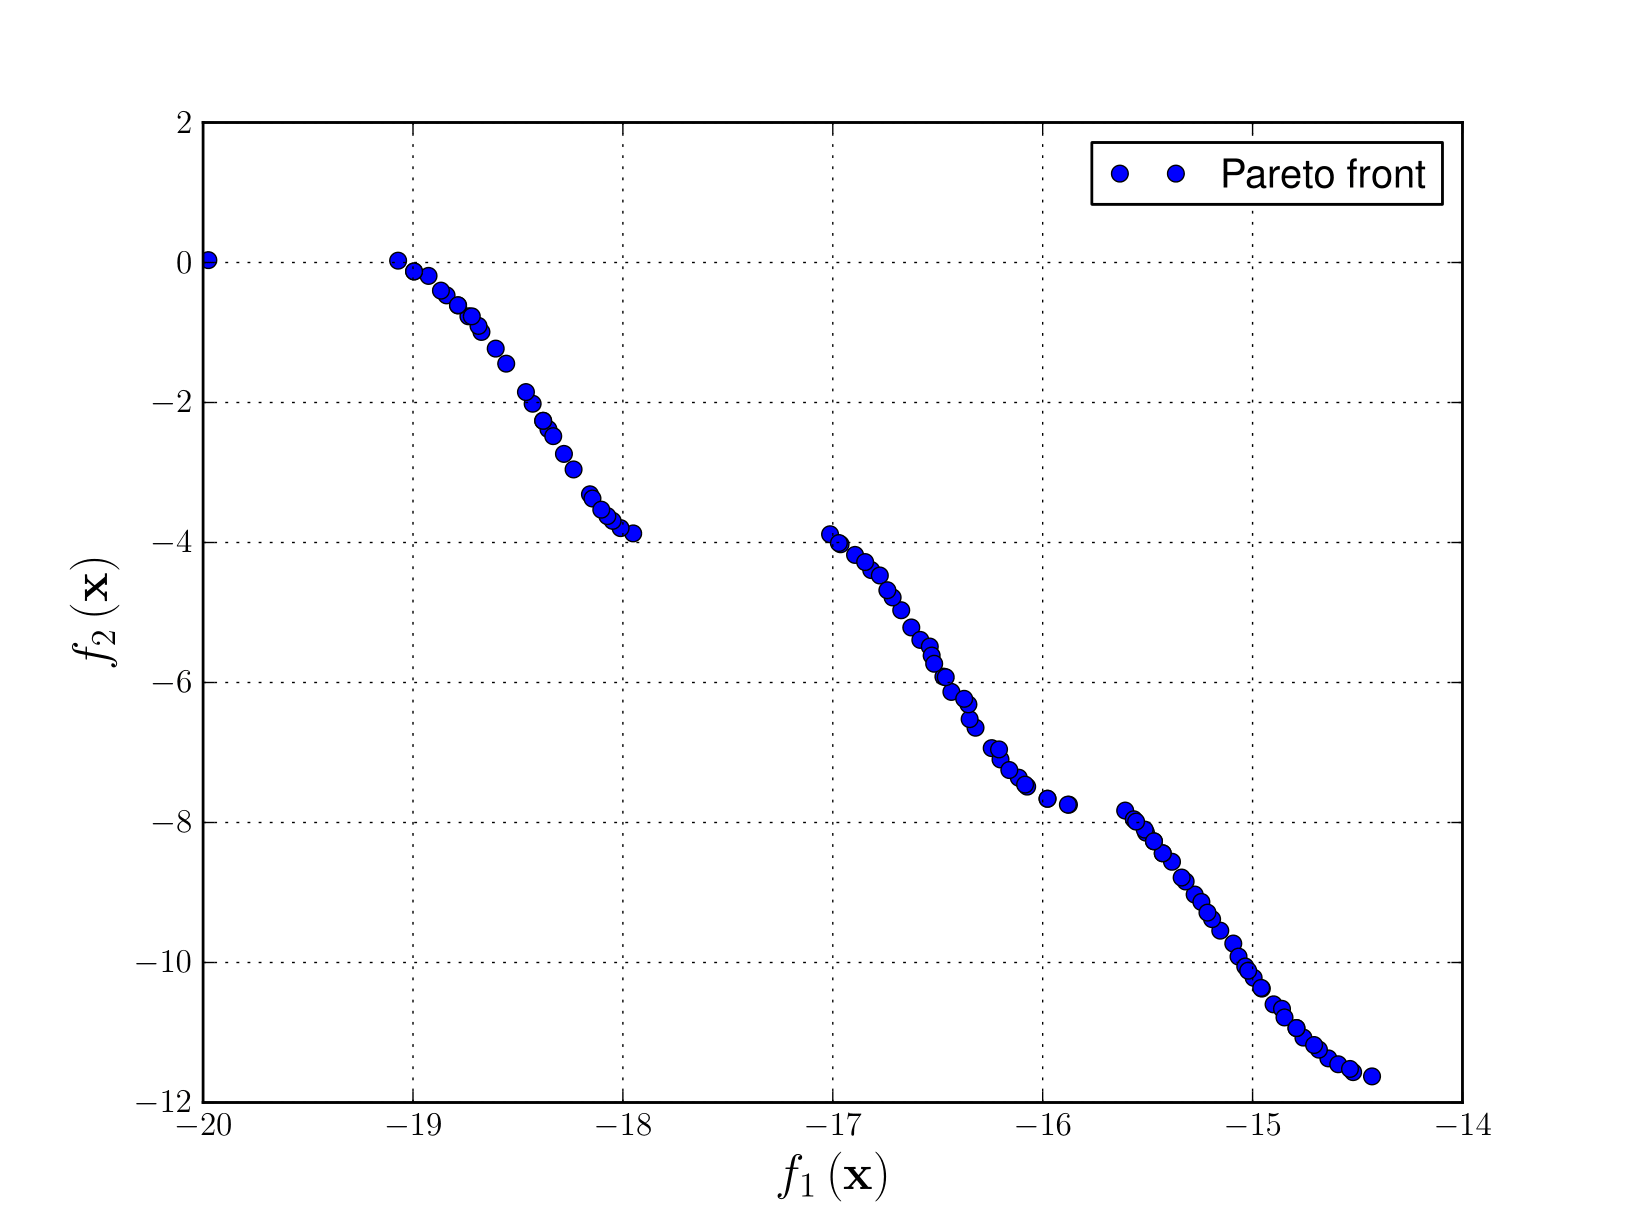
\includegraphics[width=\textwidth]{lab8/imgs/kursawe_theory.png}
        \caption{Theoretical Pareto front}
    \end{subfigure}
    \begin{subfigure}{0.5\textwidth}
        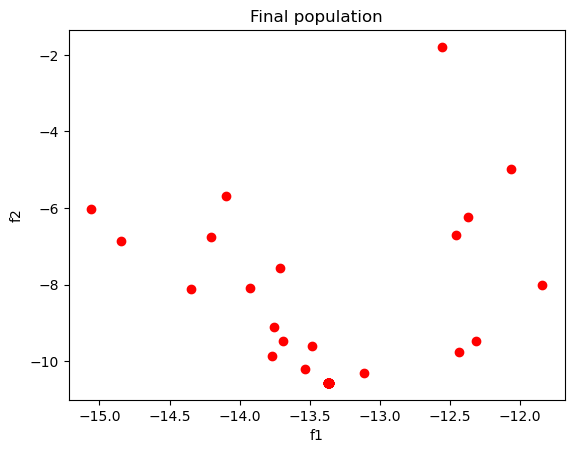
\includegraphics[width=\textwidth]{lab8/imgs/kursawe_ga.png}
        \caption{Genetic Algorithm final population}
    \end{subfigure}
\end{figure}

We also solve the Kursawe function using the NSGA-II algorithm. The algorithm is able to find a set of solutions that are close to the theoretical Pareto front. The final population, sorted in the fronts created by the algorithm, is shown below.
\begin{figure}
    \centering
    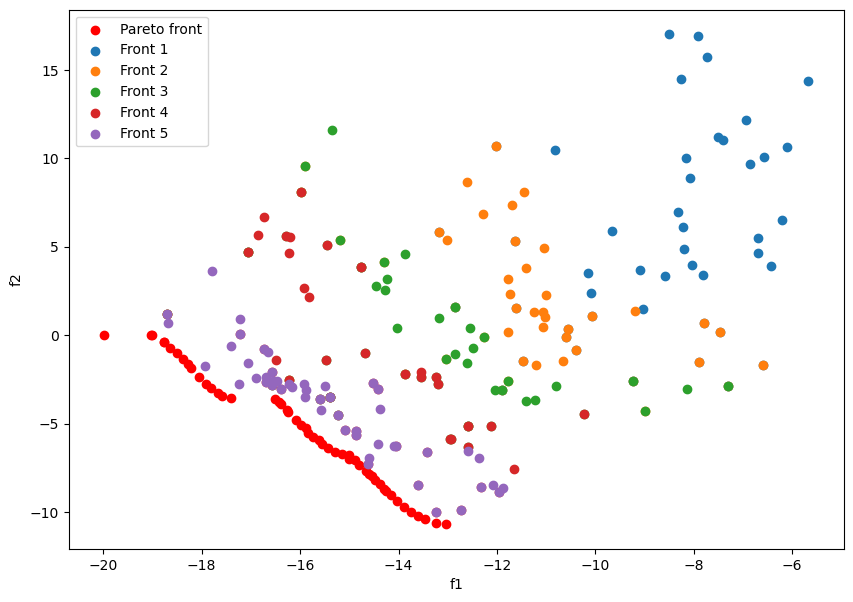
\includegraphics[width=\textwidth]{lab8/imgs/kursawe_nsga.png}
    \caption{NSGA-II final population}
\end{figure}



\subsection{Multiple-Disk Clutch Brake Optimization}
Real-world problem consisting of the optimization of five different parameters concerning the design of a multiple-disk clutch brake. The parameters are:
\begin{enumerate}
    \item $r_i \in [60,61,...,79,80]mm$ - inner radius of the disks
    \item $t_o \in [90,91,...,109,110]mm$ - outer radius of the disks
    \item $F \in [600,610,...,990,1000]N$ - force applied to the disks
    \item $t \in [1,1.5,2,2.5,3]mm$ - thickness of the disks
    \item $Z \in [2,3,4,5,6,7,8,9,10]$ - number of disks
\end{enumerate}
The two conflicting objectives are:
\begin{enumerate}
    \item minimization of the break system mass
    \item minimization of the stopping time
\end{enumerate}
We also consider an additional situation (constrained) where the fitness value of an individual is penalized every time the constraints on the range of the parameters are violated. We can see that the achieved Pareto front achive slightly better results in the constrained case specifically in the coverage of the Pareto front.
\begin{figure}[H]
    \begin{subfigure}{0.5\textwidth}
        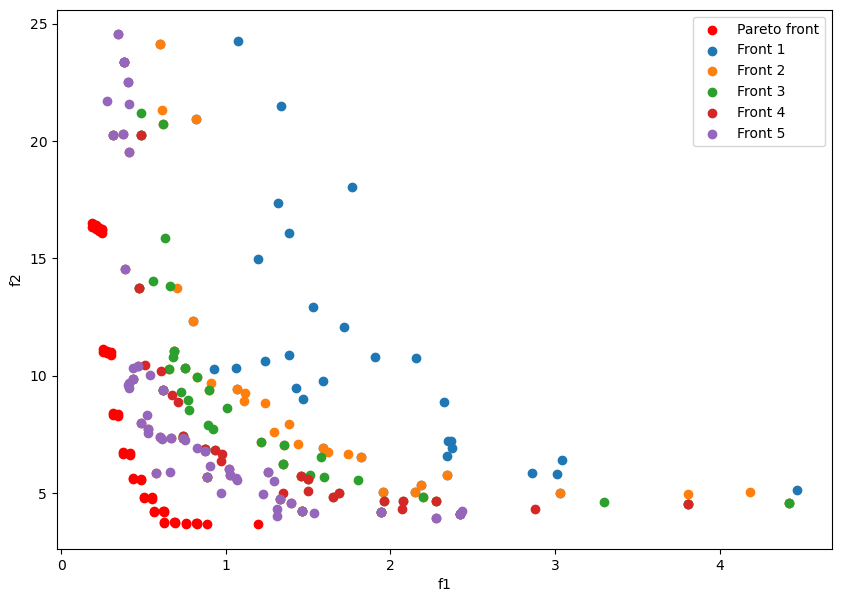
\includegraphics[width=\textwidth]{lab8/imgs/disk_nsga.png}
        \caption{NSGA-II final population}
    \end{subfigure}
    \begin{subfigure}{0.5\textwidth}
        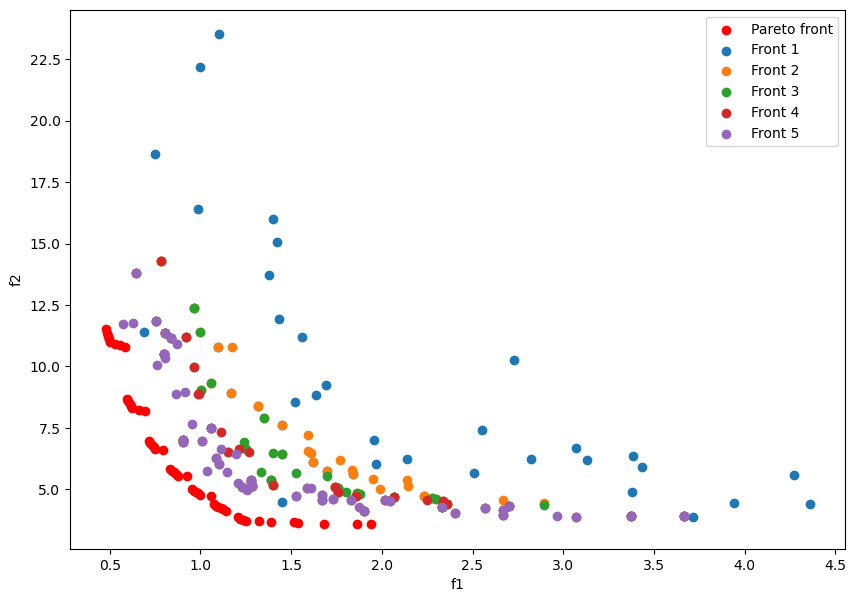
\includegraphics[width=\textwidth]{lab8/imgs/disk_constr_nsga.png}
        \caption{NSGA-II final population (constrained)}
    \end{subfigure}
\end{figure}